\documentclass{article} % For LaTeX2e
\usepackage{nips15submit_e,times}
\usepackage{hyperref}
\usepackage{url}
\usepackage{graphicx}
\usepackage{float}
\usepackage{mathtools}
\usepackage{listings}
\usepackage{bm}
\usepackage{amsmath}
\graphicspath{ {figures/} }
\DeclareMathOperator*{\argmin}{\arg\!\min}
\DeclareMathOperator*{\argmax}{\arg\!\max}
\DeclareMathOperator*{\sigmoid}{sigmoid}
\DeclarePairedDelimiterX{\norm}[1]{\lVert}{\rVert}{#1}

\renewcommand{\lstlistingname}{Listing}

\lstset{
   breaklines=true,
   basicstyle=\ttfamily}

%\documentstyle[nips14submit_09,times,art10]{article} % For LaTeX 2.09


\title{COMPGI15: Information Retrieval \& Data Mining \\
Time Series Forecasting Group Project}


\author{
Rupert Chaplin\\
\texttt{rupert.chaplin.15@ucl.ac.uk} \\
\And
Artemis Dampa\\
\texttt{artemis.dampa.15@ucl.ac.uk} \\
\And
Megane Martinez\\
\texttt{megane.martinez.15@ucl.ac.uk} \\
}


\newcommand{\fix}{\marginpar{FIX}}
\newcommand{\new}{\marginpar{NEW}}

\nipsfinalcopy % Uncomment for camera-ready version

\begin{document}


\maketitle

% No abstract needed
\begin{abstract}
placeholder for abstract
\end{abstract}

\section*{Introduction}
A time series can be defined as a set of observations measured successively over a continuous time interval. Every measurement is taken at a specific time which is equally distant to its subsequent. The analysis of time series takes into consideration the ordering of the data points and constitutes a useful tool in order to extract information such as the causal effect of time change on the variable which is examined. After describing and analysing the time series one can gain an understanding of the data and thus, define a model with the best possible fit at the data based on the past values of the examined variable and/or the past and present observations of other variables which might influence the former. Using the created model one can, finally, make predictions and forecast the future values of the examined variable or even use models to backcast and possibly fill in missing values. The ultimate goal of time series analysis is to control and manage the process involved in the time series.

Load forecasting and especially, short term load forecasting which can predict energy load values ranging from one day to one fortnight at hourly or sub hourly intervals, has always been of great importance for managing power systems. It is used in economic generation scheduling, fuel scheduling, unit commitment and system security, as well as in transmission and distribution operations. There are several machine learning methods which can be applied in order to achieve short term load forecasting, such as ARIMA, Multiple linear regression, Gradient boosting and Neural networks.

The dataset used in order to implement the time series techniques for forecasting (and backcasting) is provided by the Load Forecasting track of Global Energy Forecasting Competition 2012. The aim of the competition was to collect different approaches for energy forecasting in order to “overcome forecasting challenges in the smart grid world”. More specifically, the load forecasting track was addressing a hierarchical load forecasting problem. The goal was to use forecasting (and backcasting) in order to predict hourly loads (in kW) for a US utility with 20 zones.



\section*{Data availability}
In developing this work, we embraced the same constraints on data use imposed upon the original Kaggle challenge - confining ourselves to use of the originally provided datasets, which are:
\begin{itemize}
\item Time series for the electricity load in 20 zones, at hourly intervals between 1 January 2004 and 30 June 2008.
\item Time series of temperature readings at 11 stations, at hourly intervals over the same time period (locations not provided)
\item Dates of US holidays falling during the period
\end{itemize}
The task is to generate estimates of electricity load in each zone, and for the region as a whole, for eight hold out weeks within the period.  Additionally, forecasts are required for the week 1 July 2008 to 7 July 2008, for which no temperature readings are available.

\section*{Temperatures forecasting}
In this project, most of the implemented models, use the values provided in the temperature dataset as features for predicting energy loads values. However, the last week of temperature values is missing (2008-07-01 to 2008-07-01). Therefore, predicting the values for this week was a critical challenge for the results would impact the quality of the results provided by the implemented models.
Teams that took part in the Kaggle competition usually, used naive techniques for forecasting temperature values such as taking the average of the previous values. In this project, it was decided to use ARIMA modelling to forecast the missing temperatures. This approach represents an improvement from what has been done in the Kaggle competition and was one of the challenges to overcome.

\section*{Consideration of feature selection}
Before determining the features of the model and after performing data cleansing and editing, it is essential to create and examine the time plot of the data. The time plot can show the behavior of the data and reveal important features such as seasonal variation and trend which is defined as “an increasing normal number assigned to each observation in chronological order”.

In our case the time plot showed various fluctuations with an annual seasonality which led us to develop a set that combines several features; trend, hour with 24 levels (representing the hours of a day), weekday with seven levels (representing the days of a week), month with 12 levels (representing the months of a year), temperature of the current hour, temperature of the current hour and cubic temperature of the current hour. In addition to those main features, interaction between them was taken into account forming several cross effects; weekday$\times$hour, temperature$\times$month, temperature$^2$$\times$month, temperature$^3$$\times$month, temperature$\times$hour, temperature$^2$$\times$hour and temperature$^3$$\times$hour. After measuring the feature importance, we plotted the results as shown in Figure \ref{fig:var_imp}.
\begin{figure}
  \centering
    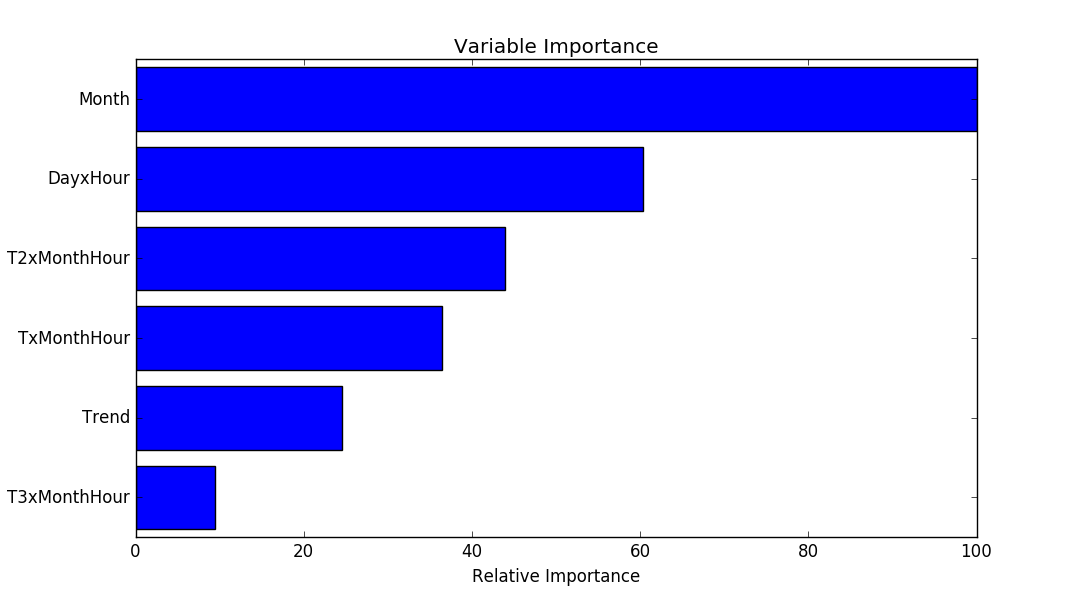
\includegraphics[width=0.80\textwidth]{variable_importance}
  \caption{Shows the feature importance measurements over the features}
  \label{fig:var_imp}
\end{figure}

\section*{Evaluation Methods}
To compare the predictive power of our models, we have adopted the same evaluation method adopted by the original Kaggle competition.  This allows us to objectively compare predictions from the different approaches we consider, and also compare out results to those achieved by those participating in the original competition.

This approach is a Weighted Root Mean Square Error, with a weighting of 1 for each zonal prediction within the period covered by training data, and a weighting of 8 for predictions within the forecast period.  Weightings of 20 and 160 are applied for each prediction of total regional load.

Root Mean Square Error is a common evaluation method for regression problems - it is a measure of average absolute distance between predicted and actual results.  It has the advantage of being expressed in the same units as that of the data we are trying to predict.  Unlike some other approaches, it is indifferent to whether overall discrepancy is due to large discrepancies on a small number of distant outliers, or due to smaller errors affecting a large number of datapoints.

The addition of weighting for this problem means that succesful models will be those which are 

Monitoring the evaluation metric also allows us to monitor models for `overfitting'.  Overfitting occurs when a model becomes tuned to the specific characteristics of a training data set, and does not generalise well to unseen test data. Overfitting would be signalled if the error measure is higher for a test dataset than it is for training data.

\section*{Modelling Approaches}

\subsection*{ARIMA}

\subsubsection*{The model}
What makes time series different from other regression problems is that they are time dependent. Therefore, instead on trying to find some correlations between the value to predict and external features, one can try to find correlations between the data points in a time series among themselves in order to predict future values. ARIMA (Auto Regressive Integrated Moving Average) is a time series modelling method that uses this approach and has become popular in the seventies.
Before we discuss how ARIMA actually works, let’s see what the prerequisites are for a time series to be effectively modelled with ARIMA.

Typically, time series can be divided into three components: the trend, the seasonality and the residuals. The trend is the long term direction of the series (upwards or downwards), the seasonality represents recurrent patterns that can be quarterly, monthly, daily and so on. The residuals are the random noise that is left after extraction of the other two components. The interference of the trend, seasonality and residuals produces the final time series.
Most of time series modelling approaches, ARIMA included, works on the assumption that the series is stationary, i.e, its mean and variance remain constant over time. In order to use ARIMA to model a time series, one needs to, first, make it stationary on both mean and variance.
One of the way of making a time series stationary on mean, is to remove the trend by using first order differencing: Y’t = Yt – Yt-1.

Most of time series become stationary after first order differencing. If the residuals time series still has a trend, one can use 2nd order differencing.
In order to make a series stationary on variance, one usually uses log transformation: Y’t = log10(Yt).
Finally, the combination of both 1st order differencing and log transformation makes a time series stationary on both mean and variance.

ARIMA is divided in three components, each with its parameter. AR stands for Auto Regressive and its parameter in p. I stands for integrated and its parameter is d and MA stands for Moving Average and its parameter is q.
As seen previously, ARIMA uses past time series data points to predict the future values. The auto regressive part of the model defines lags of dependent variable. For instance if p = 2, AR will use the past two values to predict a third one.
The parameter d of the Integrated part of the ARIMA model simply defines the order of difference. If the first order differencing is enough to make the series stationary one can use the differenced data and put k = 0 or use the original log transformed data and put k = 1.
The Moving Average part of the model defines the number of lagged errors used to predict the next value. If q = 2, its means that to predict a value the model will use the past two errors, i.e, differences between the moving average and the actual value.

\subsubsection*{Design choices}
Several statistical libraries or packages offer tools to implement ARIMA modelling. However some are more comprehensive than others. For example, in Python, the package \verb~statsmodels.tsa.arima_model~ allows one to create ARIMA modelling but does not have a way to find the parameters (p,d,q) of the best fit model automatically. The package \verb~forecast~ in R however does provide this possibility with the \verb~auto.arima()~ function.

In our team, none of us were very familiar with R so we decided to use python for the overall implementation and to use an R package (PypeR) to still benefit from R additional capabilities.

In order to check the stationarity of the time series we used the Dickey-Fuller test where the null hypothesis is that the time series is non-stationary. If the test result is below the critical value we can reject the null hypothesis and say the time series is stationary and suitable for ARIMA modelling.

Checking the effectiveness of the ARIMA models was done by plotting and analysing the ACF (Auto Correlation Fuction) and PACF (Partial Auto Correlation Function) of both the differenced and log transformed data and then the ARIMA output.

The ACF plot represents the correlation coefficient between a time series and lags of itself. For instance, by looking at an ACF plot, one can know if for any data point Yt of the serie, Yt is correlated with Yt-1, Yt-2 and so on.

The PACF plot represents the part of the correlation between two data point Yt and Yt-n that is not explained by their mutual correlation with the Yt-1 to Yt-n+1.

By differencing and log transforming the raw data and plot ACF and PACF one can see if there is still some correlation left in the residuals that would be removed by using ARIMA. Plotting the ACF and PACF on the ARIMA results allows to check that there is no more correlation in the residuals and that the ARIMA model is working well.

During this project, ARIMA was used for two purposes: predict the missing energy load values and predict the missing temperature values in order to use them as features in other prediction algorithms. 

\subsubsection*{ARIMA for loads forecasting}

At first, it was decided to try implementing ARIMA modelling directly on the energy loads time series to predict the missing values. 

However, since the energy loads dataset contains hourly data from 2004-01-01 to 2008-06-30 for 20 different zones in the United States, each of this zone needed to be treated as an independent time series. Moreover, within that time range, 8 separate weeks of data were missing for each zone and needed to be forecasted as well as the week following the last data point of the set.

Most of ARIMA modelling implementation usually assume that there is no missing data within the time range of the given time series. Since the energy loads data sets was missing 8 weeks, it required modelling every range of data in between those missing weeks as an independent time series as well.

As a result, the implemented ARIMA algorithm dealt with 9 independent time series for each zone, thus, 180 time series in total.

Although the implemented algorithm dealt with a lot of independent time series, the results were constant over them. In the following are shown results for the time series from 2004-01-01 to 2005-03-06.
The following plot represents the raw time series that does not look stationary, if the overall trend is difficult to identify, there are clearly some patterns present.

\begin{figure}
  \centering
    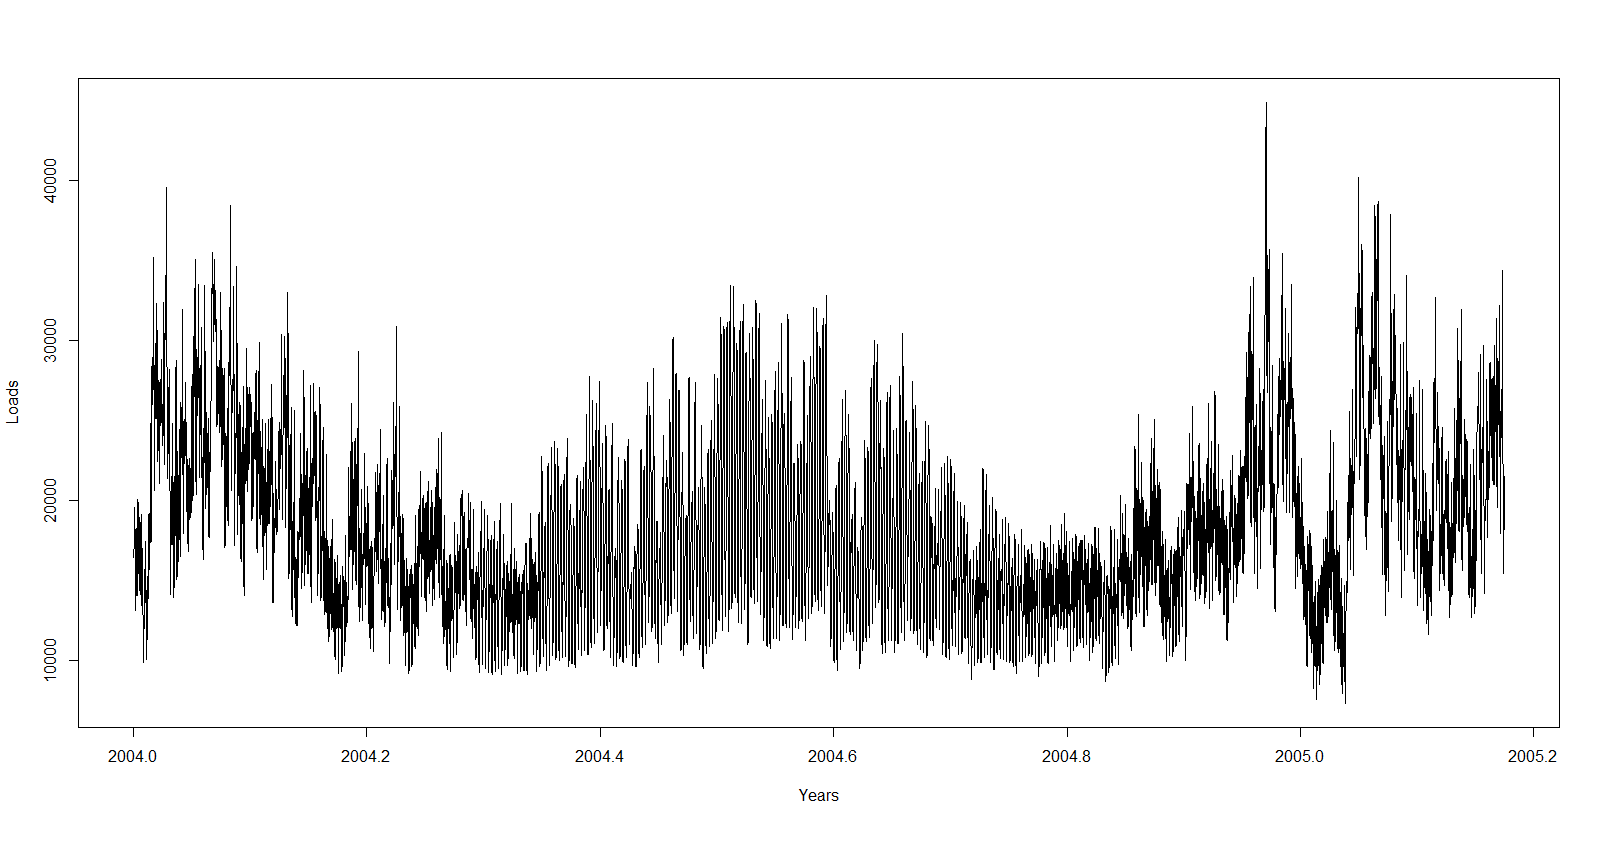
\includegraphics[width=0.80\textwidth]{loadsRawData}
  \caption{Shows the raw data for the first date range of zone 1 }
\end{figure}

The next plot represents the 1st order differenced log transformed data. This time, the series looks much more stationary. 

\begin{figure}
  \centering
    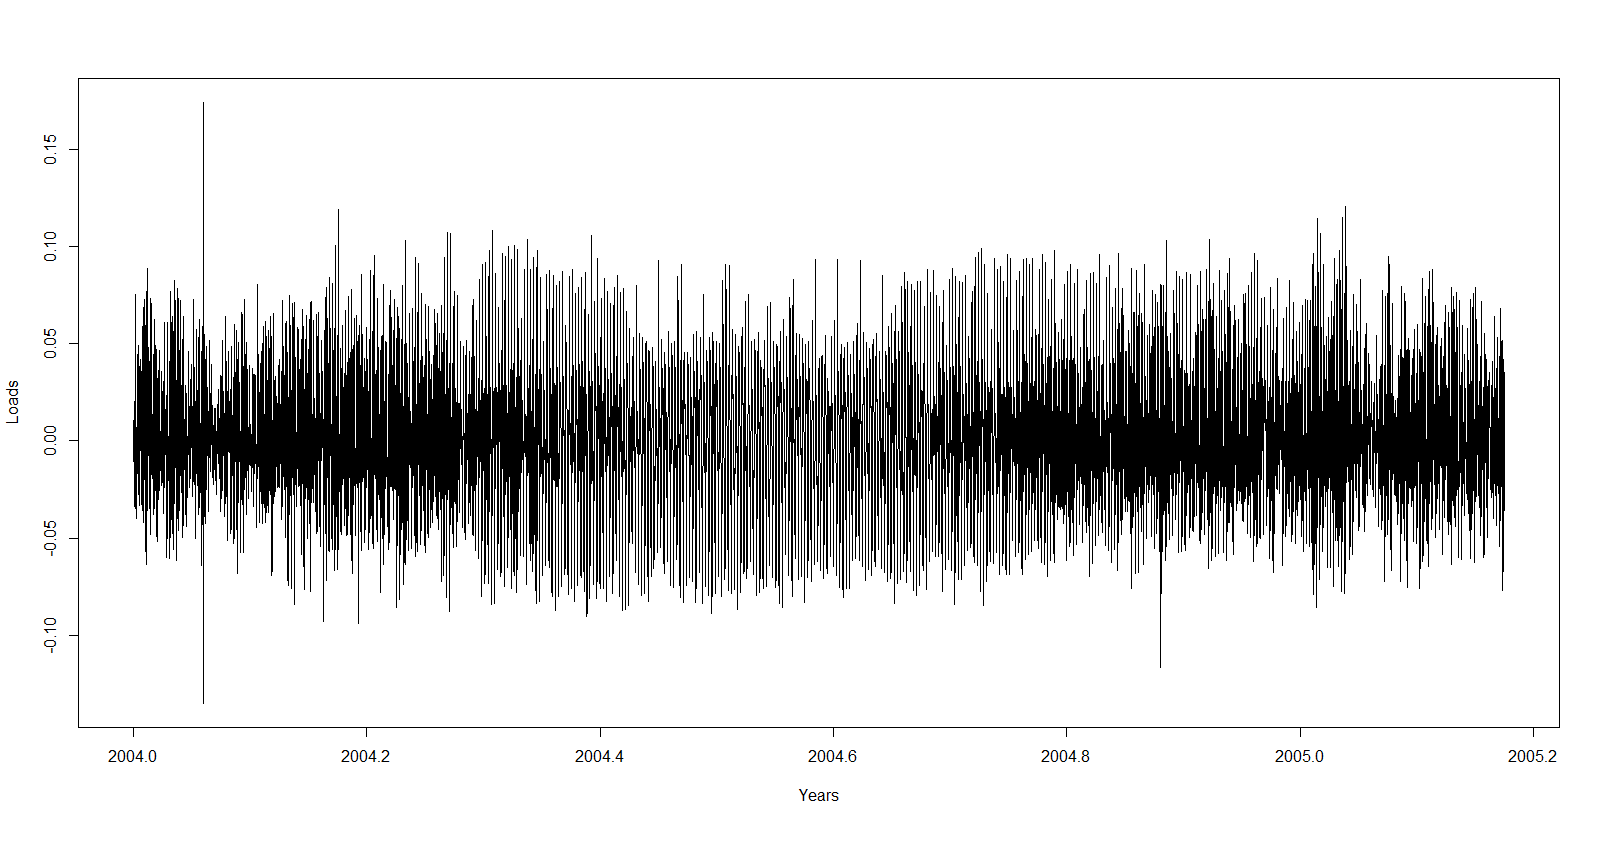
\includegraphics[width=0.80\textwidth]{LoadsStationary}
  \caption{Shows the 1st order differenced log transformed data for the first date range of zone 1 }
\end{figure}

In order to confirm that the series is stationary, the algorithm runs the Dickey-Fuller test. The output is the following:
\begin{verbatim}
Results of Dickey-Fuller Test:
Test Statistic: -1.154495e+01
p-value: 3.559772e-21
#Lags Used: 27
Number of Observations Used: 10279.000000
Critical Value 5\%: -2.861821
Critical Value 1\%:  -3.430986
Critical Value 10\%: -2.566920
\end{verbatim}

The test statistic is smaller than the critical value of 1\% which means the rejection of the non-stationarity hypothesis has less than 1\% chance to be wrong. One can conclude with confidence that the time series is stationary.

The following charts, show the ACF and PACF values of the time series. Both plots show a lot of spikes going out of the insignificant zone represented by the dotted horizontal lines. It means that the time series residuals has some information left to be extracted by the ARIMA model.
One could also notice the daily seasonality represented by the spikes at lag 24 (24 hours seasonality).

\begin{figure}
  \centering
    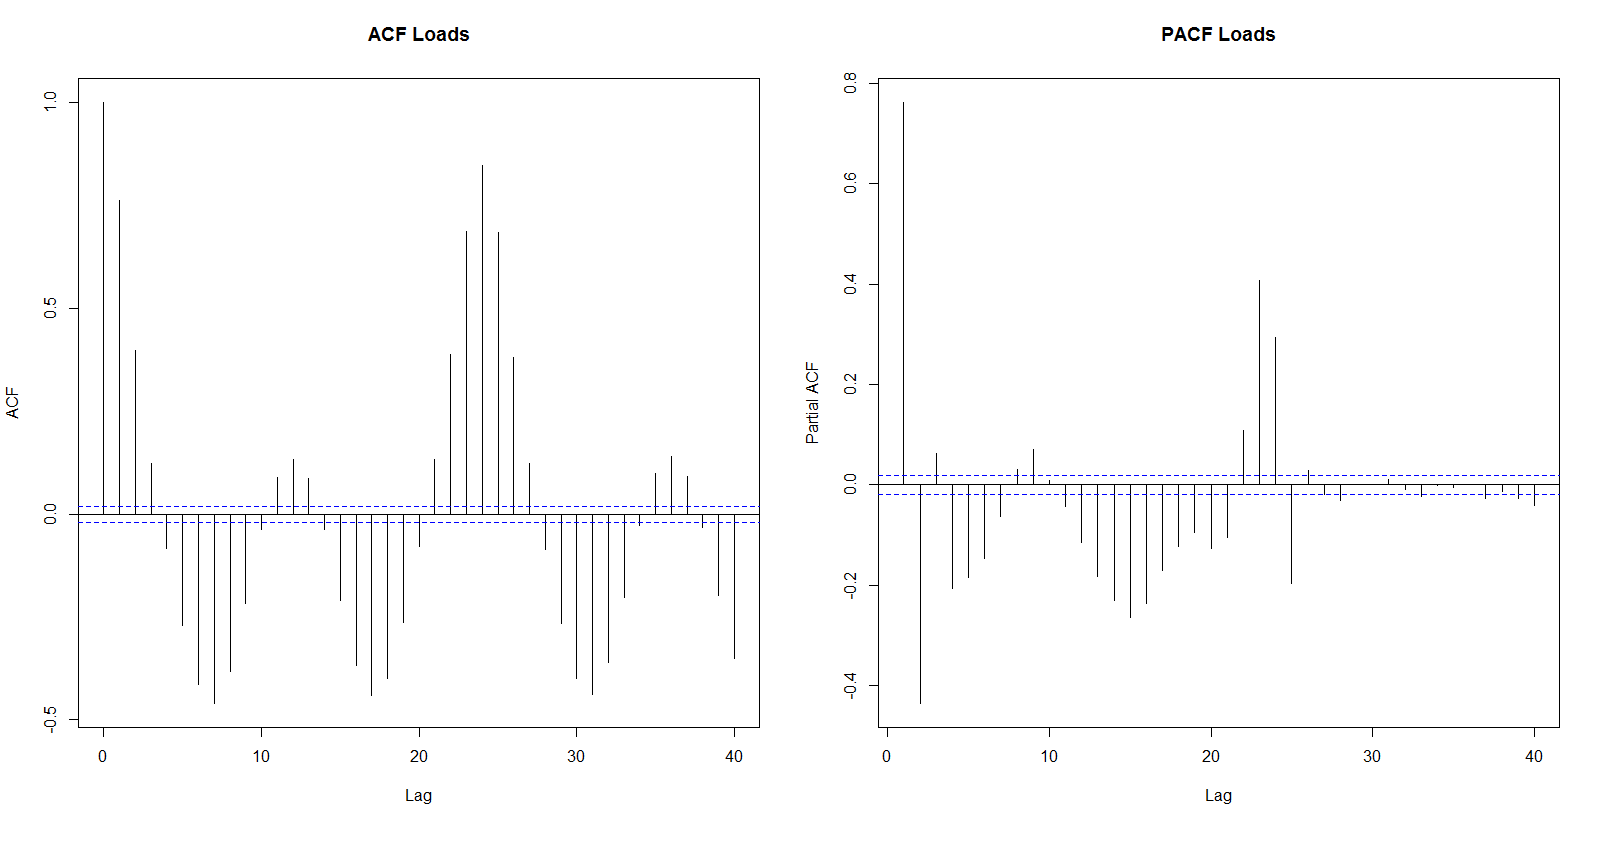
\includegraphics[width=0.80\textwidth]{ACFandPACFLoadsRaw}
  \caption{Shows the ACF and PACF values for the differenced log transformed data for the first date range of zone 1 }
\end{figure}

By using the auto.arima() function provided by R, the algorithm finds and uses the best ARIMA model for the given time series, i.e, the parameter order that provides the lowest Bayesian information criterion (BIC).
In R, one can obtain a summary of the best ARIMA model. In this case, the output was the following:
\begin{verbatim}
Series: log10(data) 
ARIMA(4,1,3)                    

Coefficients:
         ar1      ar2     ar3      ar4      ma1      ma2      ma3
      1.7072  -1.1621  0.5679  -0.2606  -0.6993  -0.1086  -0.1276
s.e.  0.0547   0.0921  0.0613   0.0229   0.0556   0.0442   0.0317

sigma^2 estimated as 0.000333:  log likelihood=26612.67
AIC=-53209.33   AICc=-53209.32   BIC=-53151.42

Training set error measures:
             ME         RMSE       MAE        MPE          MAPE      
Training set 2.2533e-05 0.01824026 0.01375096 -0.000907019 0.3242475
MASE      ACF1
0.1096394 0.001905331
\end{verbatim}

Here, the parameters of the model are p=4, d=1 and q=3 but it is important to note it was not the case for all of the independent time series the algorithm dealt with. If the d was always equal to zero, the value of p and q varied. 

The following plot represents a subset of the raw data for the given time series in black and the predicted values for the following week in blue. One can see that the first predicted values reflect some of the variation from the actual time series but then the remaining values become linear quickly.

\begin{figure}
  \centering
    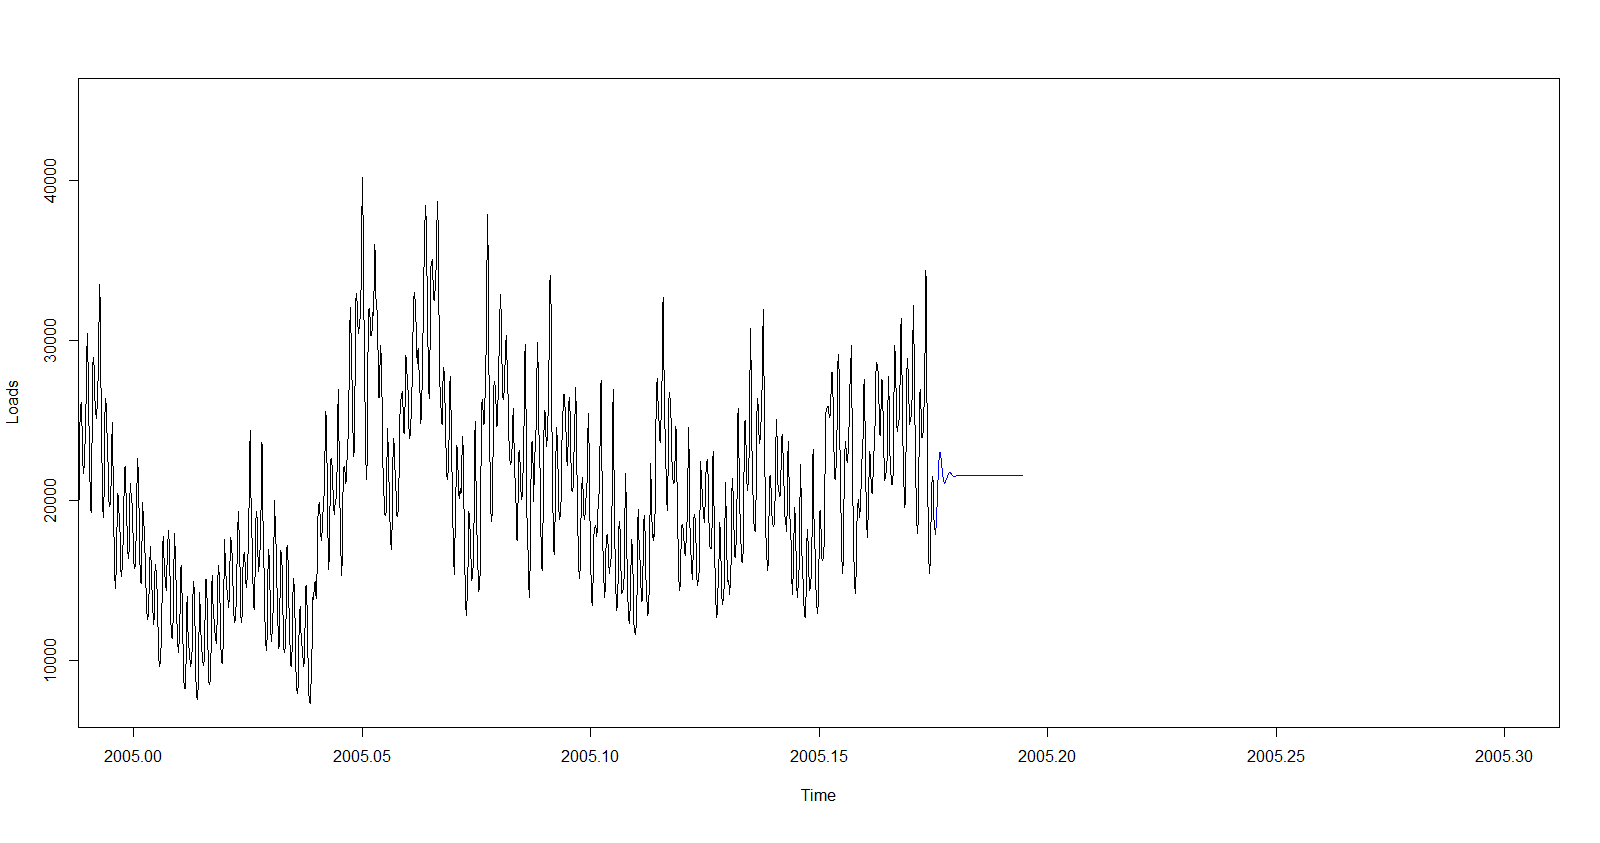
\includegraphics[width=0.80\textwidth]{LoadsPred}
  \caption{Shows predicted values for the week after for the first date range of zone 1 }
\end{figure}

If one plots the ACF and PACF of our best fit ARIMA model, one can see that although the spikes are less pronounced, some of them are still out of the insignificant zone which means that there is still information left in the residuals and explains why the model does not produce very good results.

\begin{figure}
  \centering
    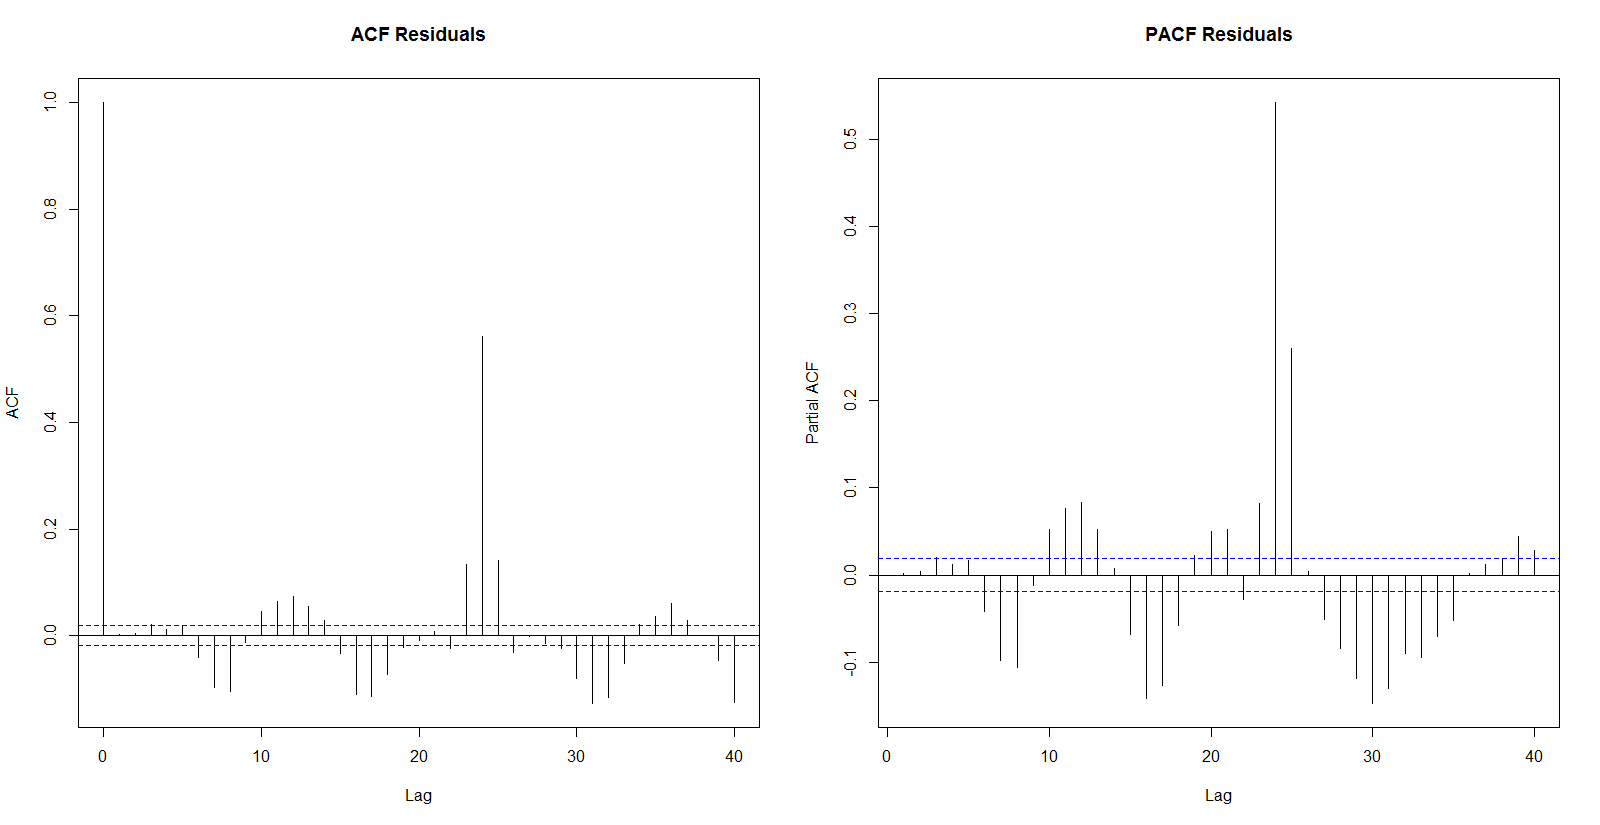
\includegraphics[width=0.80\textwidth]{ACFandPACFLoadsArimaResults}
  \caption{Shows ACF and PACF values for the ARIMA residuals for the first date range of zone 1 }
\end{figure}

The results of the implemented ARIMA model for energy loads could come from several reasons. First, the fact that the algorithm dealt with several independent time series for the same zone in order to deal with missing values might have result in a loss of information. As said before, the best fit ARIMA model was not the same for each independent time series. Without the missing values the algorithm would have dealt with only one time series per zone and it would have been possible to see the bigger picture instead of focusing one smaller ranges.

The second reason why the ARIMA did not work very well might be because the data were too detailed. Indeed, measuring the energy loads hourly over four years produces a lot of information and a lot of white noise which could explain why there was information left in the residuals of the best fit model. Finally, some time series are simply not suitable for ARIMA modelling and some other approaches need to be considered.


\subsubsection*{ARIMA for temperature forecasting}

The second try of ARIMA modelling was for the temperatures predictions. In addition to the energy data set, the temperature data set provided hourly temperature measurements for 11 different stations from 2004-01-01 to 2008-06-30 without missing values. This data set was used in other algorithms with the temperatures as features of the value to predict (energy load). One of the weeks for which to predict the energy loads was the one at the end of the data set (2008-07-01 to 2008-07-01). The temperatures for this week were not provided, thus it was necessary to predicted them in order to pass them to our energy loads predictive algorithms.

This time, the implemented ARIMA model dealt with only one time series per zone which was less tedious than for the energy loads model.

The results of the ARIMA modelling were constant across the different zones. As an example are presented the results for the station number 1.
The following charts represents the raw temperature data with the very clear yearly pattern but no noticeable trend.

\begin{figure}
  \centering
    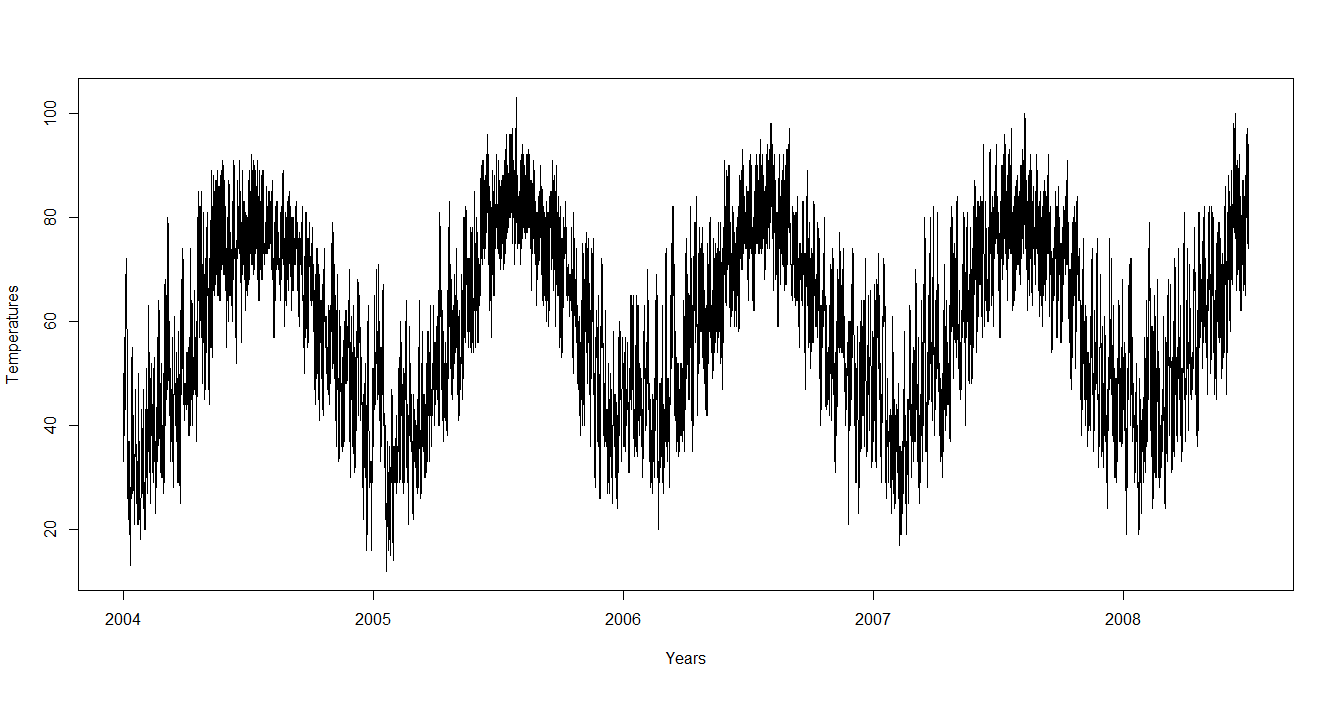
\includegraphics[width=0.80\textwidth]{TempRawData}
  \caption{Shows the raw temperature data for station 1 }
\end{figure}

Then the time series is made stationary with 1st order differencing and log transformation. The results are shown in the following plot.

\begin{figure}
  \centering
    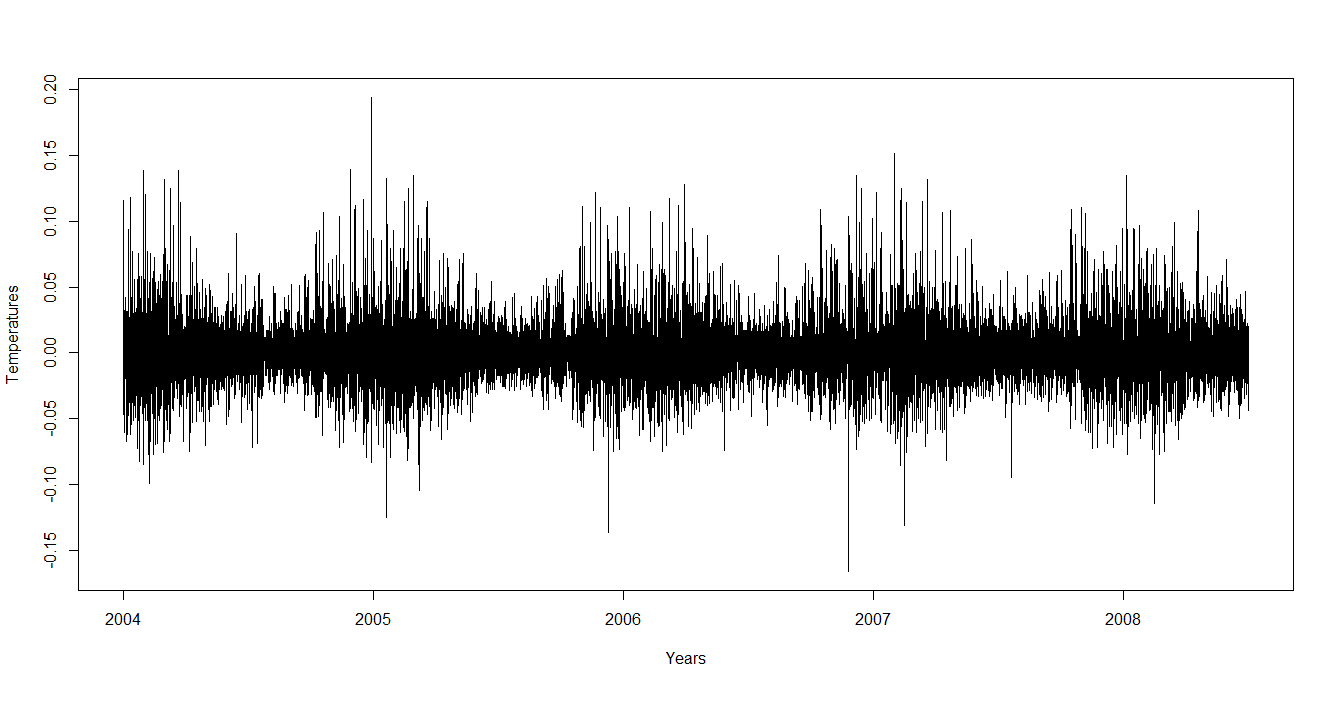
\includegraphics[width=0.80\textwidth]{TempStatData}
  \caption{Shows the 1st order differenced log transformed temperature data for station 1 }
\end{figure}

The Dickey-Fuller test was used to check if the transformed series was indeed stationary with following output:
\begin{verbatim}
Test Statistic: -33.513700
p-value: 0.000000
#Lags Used: 54.000000
Number of Observations Used: 39358.000000
Critical Value 5\%:  -2.861613
Critical Value 1\%: -3.430516
Critical Value 10\%: -2.566809
\end{verbatim}

The test statistic is smaller than the critical value of 1\% so one can assume that the series is stationary.

On the following charts one can observe the ACF and PACF values of the series. Here as well, several spikes are going out of the insignificant zone which means there is information to exploit for the ARIMA model.

\begin{figure}
  \centering
    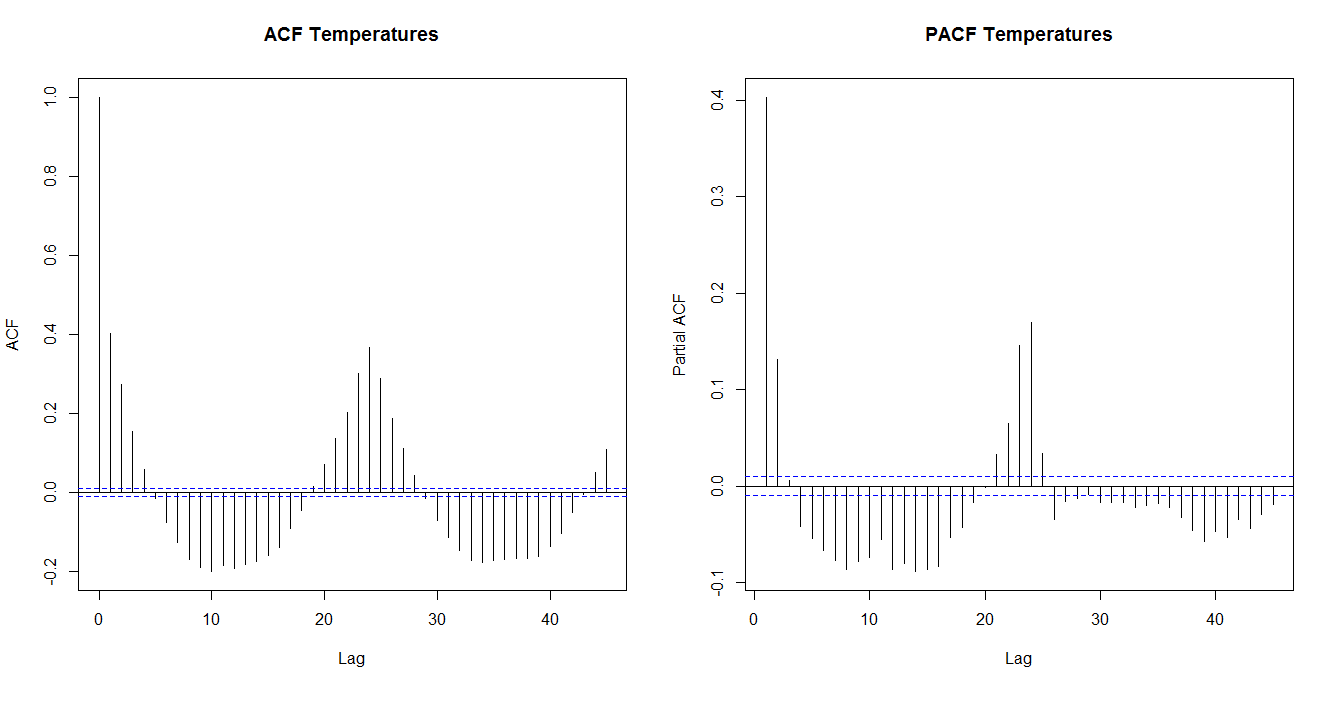
\includegraphics[width=0.80\textwidth]{ACFandPACFTempRaw}
  \caption{Shows the ACF and PACF values for station 1 }
\end{figure}

Like for the energy loads time series the auto.arima() R function gives the best fit model for the given time series, the summary of this model is the following output:

\begin{verbatim}
Series: log10(data) 
ARIMA(2,1,2)                    

Coefficients:
         ar1      ar2      ma1     ma2
      1.7959  -0.8652  -1.5442  0.5978
s.e.  0.0072   0.0071   0.0128  0.0128

sigma^2 estimated as 0.0002299:  log likelihood=109173.7
AIC=-218337.4   AICc=-218337.4   BIC=-218294.4

Training set error measures:
             ME           RMSE       MAE        MPE          MAPE
Training set 8.343304e-06 0.01516216 0.01011681 -0.004802065 0.596134
MASE      ACF1
0.1328162 0.03907321
\end{verbatim}

The parameters of the model are p=2, d=1 and q=2.

The following plot represents a subset of the raw data for the given temperature time series in black and the predicted values for the following week in blue. One can see that, just like the predictions of energy loads, the first predicted values reflect some of the variation from the actual data but then the remaining values become linear quickly.

\begin{figure}
  \centering
    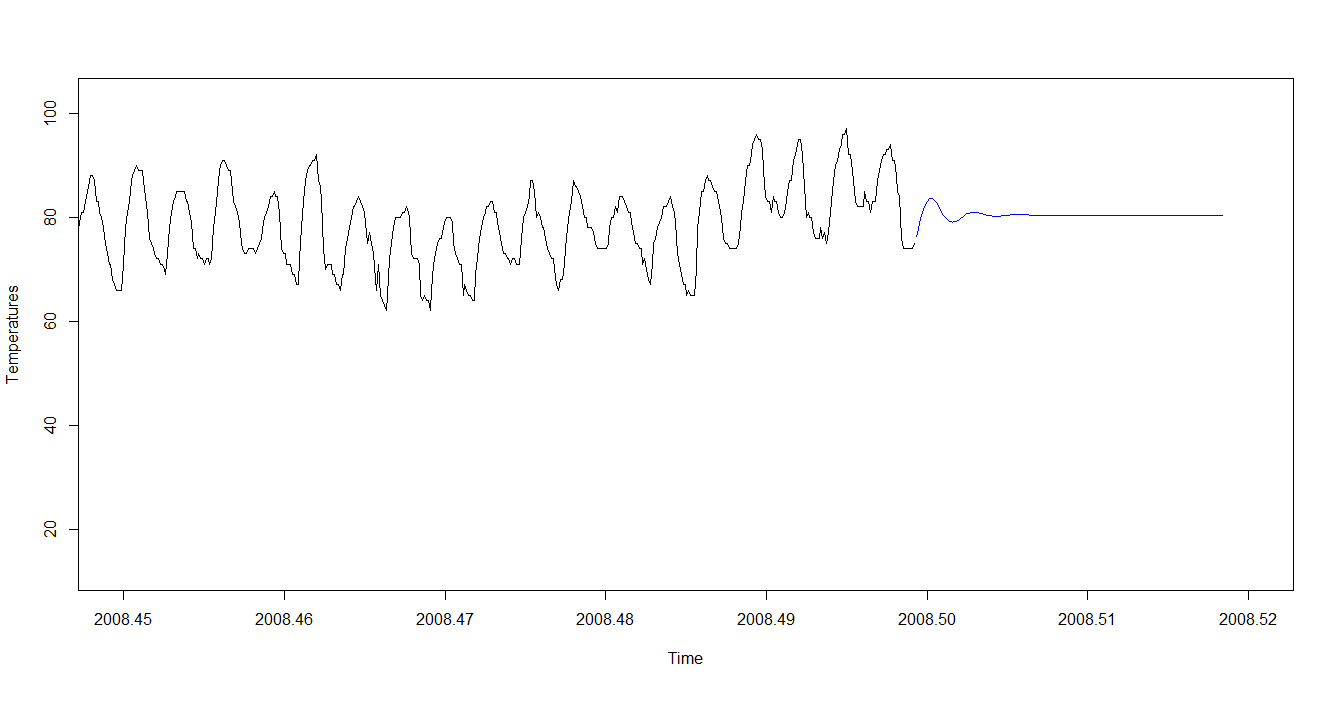
\includegraphics[width=0.80\textwidth]{TempPredictions}
  \caption{Shows predicted values for the week after the end of the data set for station 1 }
\end{figure}

This last plot shows the ACF and PACF values of the residuals of the ARIMA model. One can see that a lot of spikes are going out of the insignificant zone which means there is information left to extract and that the best fit ARIMA model is not working well.

\begin{figure}
  \centering
    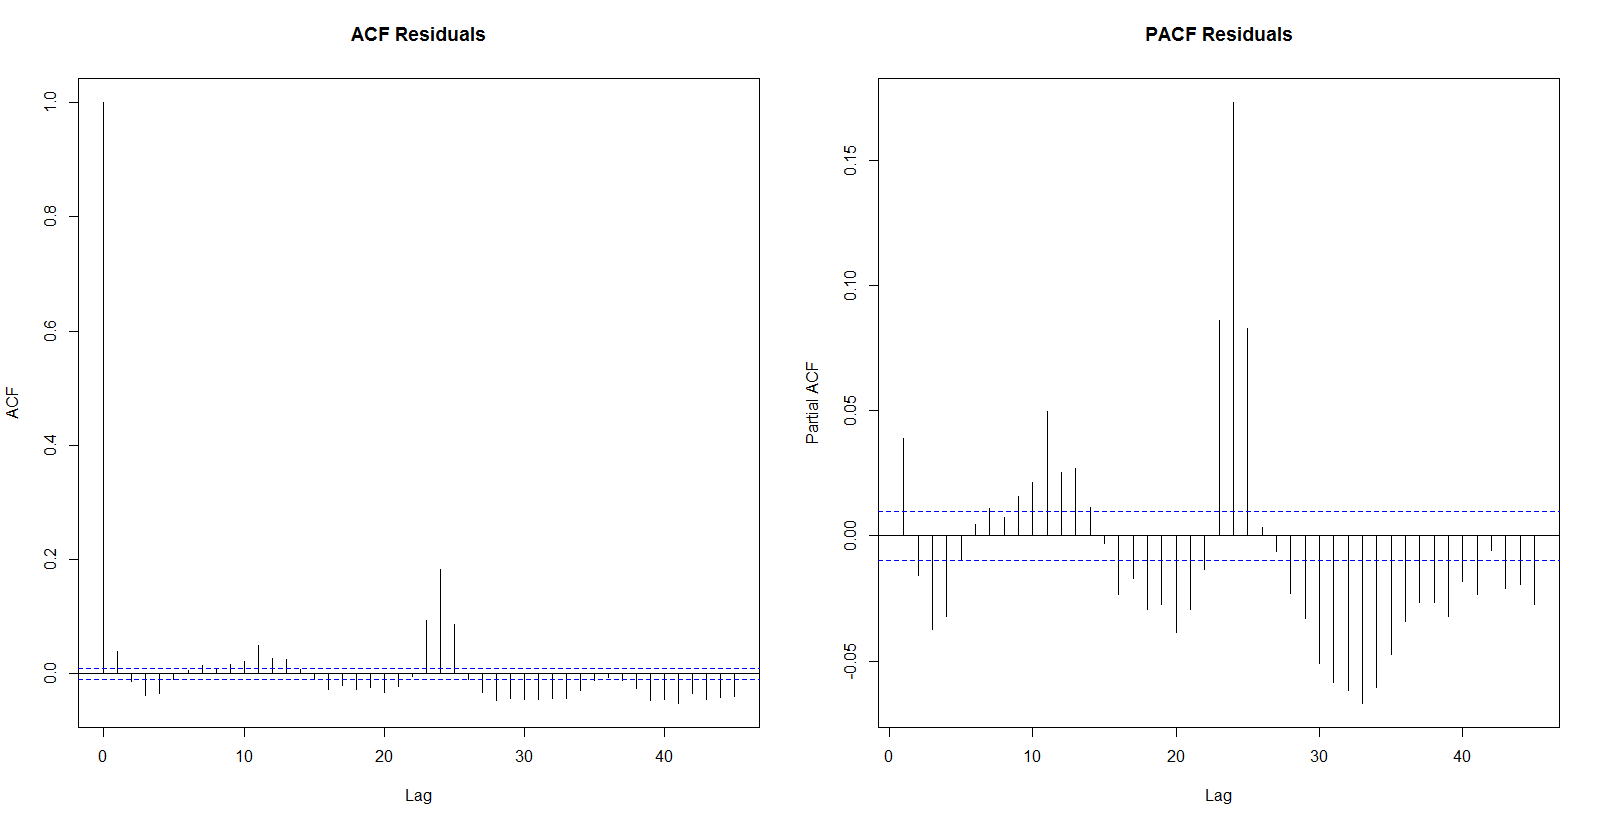
\includegraphics[width=0.80\textwidth]{ACFandPACFTempArimaResults}
  \caption{Shows ACF and PACF values for the ARIMA residuals for station 1 }
\end{figure}

As it has been said before, maybe the ARIMA did not work very well because the data were too detailed. Indeed, measuring the temperatures hourly over four years produces a lot of information and a lot of white noise which could explain why there was information left in the residuals of the best fit model. This time series might not be a good fit for ARIMA modelling.

\subsection*{Multiple Linear Regression}

\subsection*{Gradient Boosting}
Gradient Boosting is an ensemble learning method which builds additive regression models in a forward stage-wise manner. In each stage it fits a parameterised base learner to the gradient of the loss function which decreases in regard to the model values of every training sample. Gradient boosting can handle and process various data types and many different features. The factor of randomisation of gradient boosting also improves its accuracy and execution speed. Moreover, through its robust loss functions it can eliminate noise by removing outliers and thus, prevent the training model from overfitting to the data samples.

In our approach, a set of features was introduced to the gradient boosting regression model in order to best fit the data. The features are composed by the month (1-12), weekday (1-7), hour (1-24), summer (true-false), trend, holiday falling and the temperature measurements of each of the 11 temperature stations. After training the model the root mean squared error of the testing was generated and was approximately equal to 76676 whilst its weighted root mean squared error was approximately equivalent to 112081. Finally, the error of the training set and test set was computed at each iteration and can be summarised in Figure \ref{fig:deviance}, whilst the importance of all features was measured and can be observed in Figure \ref{fig:boost_imp}.
\begin{figure}
  \centering
    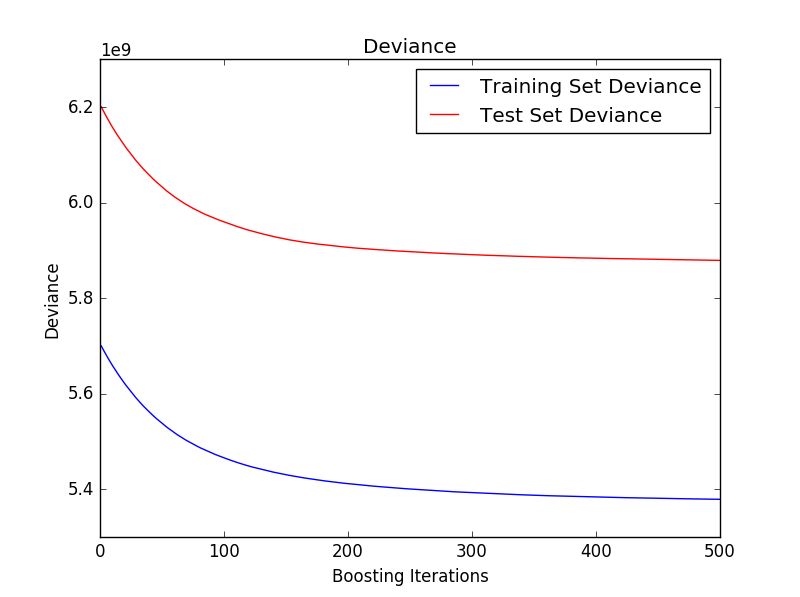
\includegraphics[width=0.80\textwidth]{deviance}
  \caption{Shows the deviance of the training and test set in gradient boosting}
  \label{fig:deviance}
\end{figure}
\begin{figure}
  \centering
    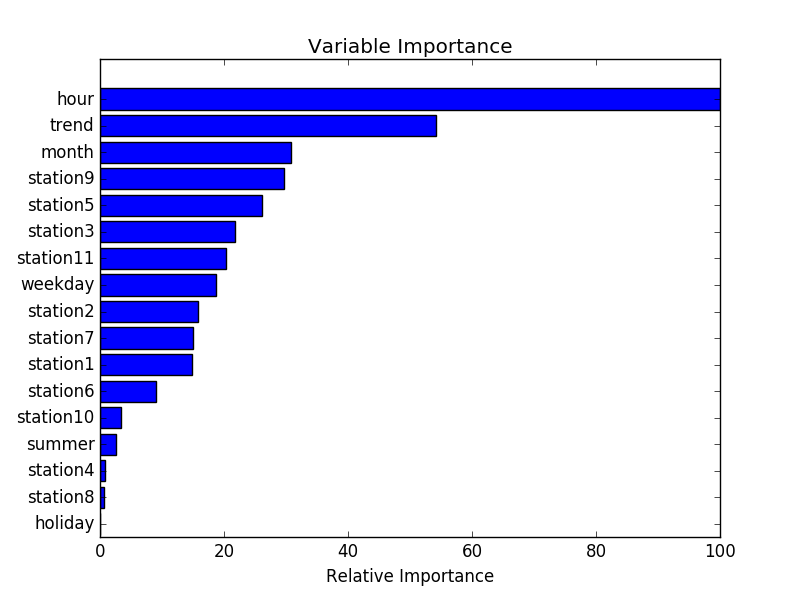
\includegraphics[width=0.80\textwidth]{boost_imp}
  \caption{Shows the feature importance measurements over the features in gradient boosting}
  \label{fig:boost_imp}
\end{figure}


\subsection*{Neural Networks}

\section*{Comparative Results}

\section*{Conclusions}


\section*{References}
\url{https://www.kaggle.com}

%\url{https://www.kaggle.com/c/global-energy-forecasting-competition-2012-load-forecasting}

Chatfield, Chris. Time-series forecasting. CRC Press, 2000.

Friedman, Jerome H. "Stochastic gradient boosting." Computational Statistics \& Data Analysis 38.4 (2002): 367-378

Hong, Tao, Pierre Pinson, and Shu Fan. "Global energy forecasting competition 2012." International Journal of Forecasting 30.2 (2014): 357-363.

Taieb, Souhaib Ben, and Rob J. Hyndman. "A gradient boosting approach to the Kaggle load forecasting competition." International Journal of Forecasting 30.2 (2014): 382-394.

\end{document}
